\chapter{Fatigue due to Environmental Loads}
\label{chap:fatigue}
In the case of a floating wind turbine, environmental loads that work on the model include waves, wind, current and more. In this thesis, the focus is on wave loads and current. Due to the cyclic nature of waves, failure of dynamic power cables applied in offshore wind farms can either be caused by overloading or fatigue.  This study focuses on failure due to fatigue. This section demonstrates the basic principles on how waves can yield fatigue damage for a dynamic power cable attached to a floating wind turbine, as can be seen in the simple flowchart in Figure \ref{fig:flowchart}. 

\begin{figure}[h!]
\centering
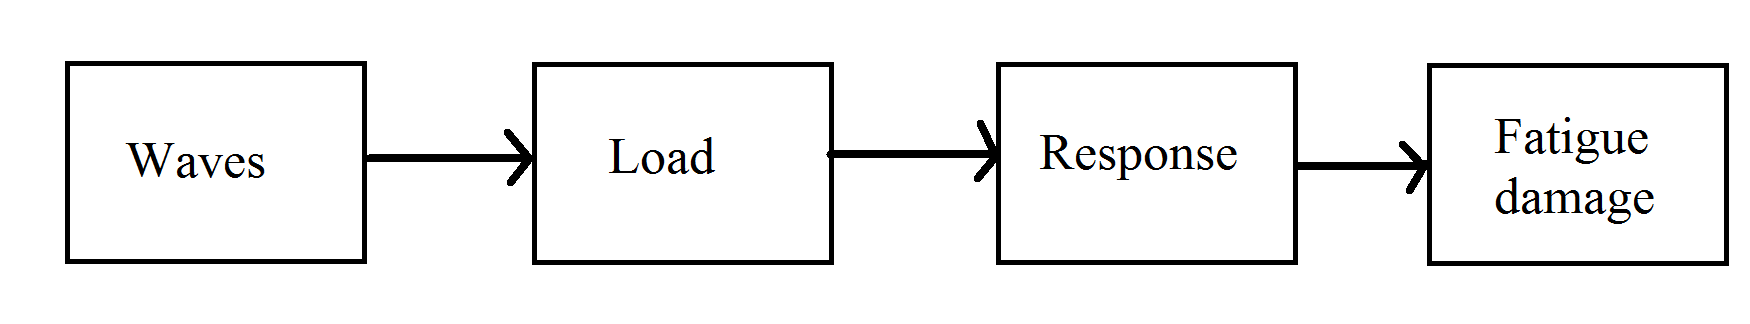
\includegraphics[scale=0.75]{figures/box}
\caption[$\; \:$Flowchart of how waves can give fatigue damage in floating structures]{Flowchart of how waves can give fatigue damage in floating structures}
 \label{fig:flowchart}
\end{figure}

\section{Statistical Description of Waves} 
 The theory in this section is taken from \cite{Faltinsen1990}.\\\\ For linear theory, the results from irregular waves can be obtained by adding together results from regular waves. For long-crested irregular sea, the wave elevation can be described as:
\begin{equation}
    \zeta = \sum_{j-1}^N A_j \sin(\omega_jt-k_jx+\epsilon_j)
    \label{eq:elevation}
\end{equation}
Where $\omega$ is the circular frequency, $t$ is time, $k$ is the wave number, $\epsilon$ is phase and $A$ is the the amplitude. $A$ can also be expressed in terms of the wave spectrum:
\begin{equation}
    \frac{1}{2}A_j=S(\omega_j) \Delta \omega
\end{equation}
Where $\Delta \omega$ is the difference between successive frequencies. The wave elevation is Gaussian distributed with mean at zero and variance at $\sigma^2= \int_0 ^ \infty S(\omega) d\omega $.\\\\ The wave spectrum assumes that the sea can be described as a stationary random process, implying that it is a short-time description of the sea state. The sea state is defined by the significant wave height, Hs, and the peak period, Tp. Hs is the mean height of the $\frac{1}{3}$ highest waves in the sea state, and Tp is the peak frequency of the wave spectrum. There exist several different specters but according to \cite{Lifes50+D1.1}: "[...]the JONSWAP (Joint North Sea Wave Project) is suitable for "wind seas," and thus used in this study. Figure \ref{fig:spectrum} show a general wave spectrum and the JONSWAP spectrum. The JONSWAP spectrum can be described as:
\begin{equation}
    S(\omega)=155 \frac{H_s^2}{T_1^4 \omega ^5} \exp{(\frac{-994}{T_1^4 \omega ^4})} 3.3^Y
\end{equation}
Where
\begin{equation}
    Y= \exp \left(-\left( \frac{0.191 \omega T_1 -1}{2^\frac{1}{2} \sigma} \right)^2\right)
\end{equation}

\begin{figure}[H]
\subfloat[General Wave Spectrum \label{fig:lm_total}]
  {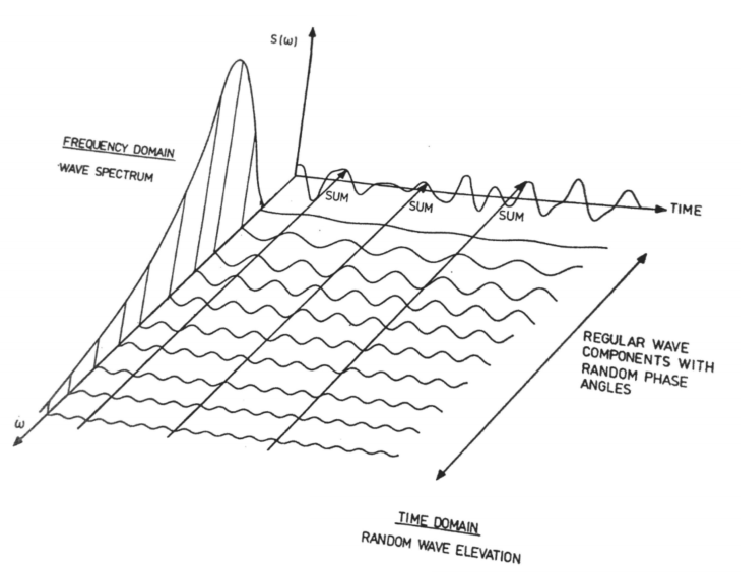
\includegraphics[width=.45\linewidth]{figures/spectrum}}\hfill
\subfloat[JONSWAP Wave Spectrum \label{fig:lm_cross}]
  {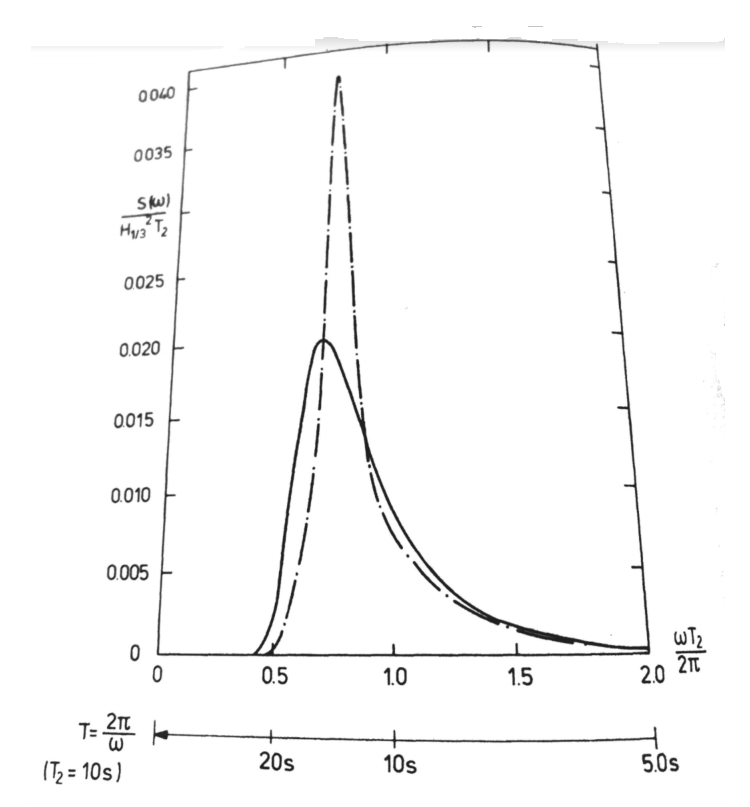
\includegraphics[width=.35\linewidth]{figures/JONSWAP}}\hfill
\caption[$\; \:$General wave spectrum and JONSWAP Spectrum]{General wave spectrum and JONSWAP Spectrum, \cite{Faltinsen1990}}
\label{fig:spectrum}
\end{figure}

\noindent The long-term sea state is usually described in a scatter diagram featuring the number of occurrences for different Hs and the Tp.\newline

\section{Load from Waves}
The loads from the waves acting on the floating wind turbine can be calculated using Morison's Equation. The general Morison's Equation expresses the horizontal force dF on a strip of the length dz of a fixed vertical cylinder and is formulated in \cite{BP2007} as:
\begin{equation}
    dF=\rho \frac{\pi D^2}{4} C_M a_x dz +\frac{1}{2} \rho C_D Du |u|dz
    \label{eq:morison}
\end{equation}
\noindent Where $\rho$ is the density of the water, D is the diameter of the pipe, $C_M$ is the mass coefficient, $a_x$ is the horizontal particle acceleration, is the acceleration in x direction, $C_D$ is the drag coefficient and u is the horizontal particle velocity. \newline
\newline
\newline
In the case of a moving cylinder, the Morison's Equation can be modified according to \cite{Faltinsen1990} as follows:
\begin{equation}
    dF=\frac{1}{2}\rho C_D D dz(u-\dot{\eta_1}) |u-\dot \eta_1| +  \rho C_M \frac{\pi D^2}{4} dz a_1 -\rho (C_M-1) \frac{\pi D^2}{4} dz \ddot{\eta_1}
    \label{eq:movemorison}
\end{equation}
Where $u$ and $a_1$ depend on position and dot represents time derivative.
\section{Response}
\cite{Langen1999} explains that an arbitrary loading can be written as a sum of harmonic components, and these can be Fourier-Transformed so that the contribution from each of the components will be a function of $\omega$. The response can also be transformed into the frequency domain, and this will give a direct measure of how the structure responds to different load frequencies as in Figure \ref{fig:transex}. "Solution in the frequency domain is particularity suited for analysis of the response to stochastic loads [...]" \cite{Langen1999}. 
 
\begin{figure}[H]
\subfloat[Transformed excitation\label{fig:transex}]
  {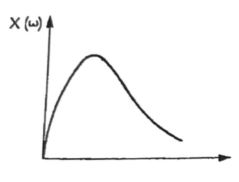
\includegraphics[width=.3\linewidth]{figures/transex}}\hfill
\subfloat[Transfer function \label{fig:cavS2500}]
  {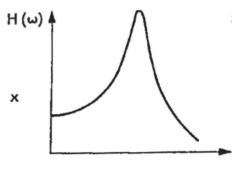
\includegraphics[width=.3\linewidth]{figures/transex2}}\hfill
  \subfloat[Transformed response \label{fig:cavS5000}]
  {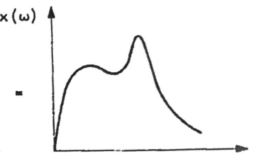
\includegraphics[width=.3\linewidth]{figures/transex3}}\hfill
\caption[$\; \:$Solution in the frequency domain]{Solution in the frequency domain, \cite{Langen1999}}
\label{fig:transex}
\end{figure}

\noindent Motion transfer functions provide an efficient description of the motion characteristics of a floating vessel. They are calculated for all 6 degrees of freedom on a specified point on the vessel from either potential theory or experimental tests, \cite{sintef2017}. Due to linearity, the response can be analyzed for each wave component in Equation \ref{eq:elevation} separately, \cite{Faltinsen1990}. Recalling Equation \ref{eq:elevation}, for wave elevation, the steady state response can be written as:

\begin{equation}
    A_j |H(\omega)|\sin(\omega_jt-\delta_j(\omega)+\epsilon_j)
\end{equation}
Where $|H(\omega)|$ is called the transfer function. For irregular sea, the response can be linearly superposed for all the different wave components:
\begin{equation}
    \sum_{j=1}^N  A_j |H(\omega)|\sin(\omega_jt-\delta_j(\omega)+\epsilon_j)
\end{equation}
 $|H(\omega)|$ and $\delta(\omega_j)$ are functions of frequency, $\omega$.\\\\
For the global model in SIMA RIFLEX, the transfer functions of OO-Star have been provided by Dr. Techn. Olav Olsen, to simulate the motions of the vessel when subjected to waves. As the transfer functions are regarded as confidential they cannot be reproduced in this report.   

\section{Fatigue}
Fatigue is damage due to cyclic loading over time where the stress is usually lower than the yield stress for a given material. In this section, some fundamental concepts related to fatigue are presented, as well as some methods used in this master thesis. The following is taken from the compendium by \cite{fatigue2016}. 
\subsection{Basic Concepts}
In Figure \ref{fig:fatigue}, some basic concepts are defined. 

\begin{figure}[h!]
\centering
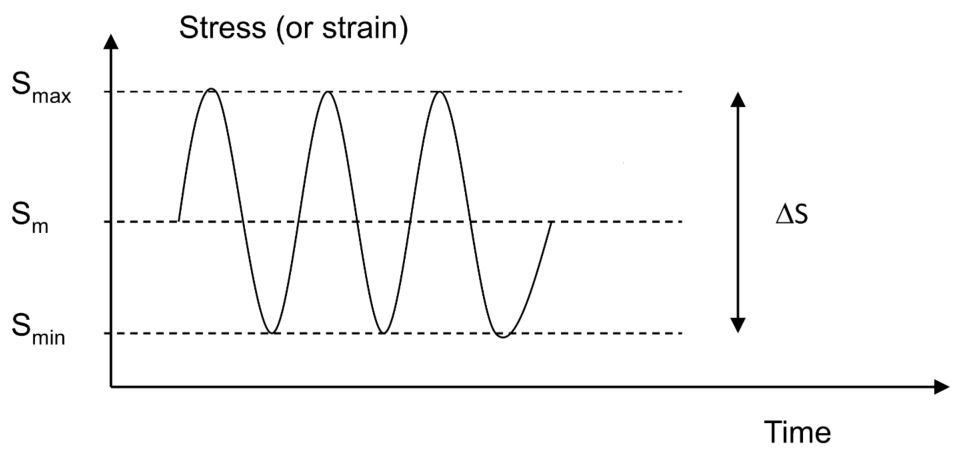
\includegraphics[scale=0.6]{figures/cycle}
\caption[$\; \:$Example of a fatigue load history]{Example of a fatigue load history, reproduced from  \cite{fatigue2016} }
 \label{fig:fatigue}
\end{figure}

From Figure \ref{fig:fatigue}, it can be seen that:
\begin{itemize}
    \item $\sigma_{max}$ -  Maximum stress/strain in a cycle
    \item $\sigma_{min}$ -  Minimum stress/strain in a cycle
    \item $\sigma_{m}$ - Mean stress/strain in a cycle
\end{itemize}

moreover, it follows that the stress range, $\Delta \sigma$ is:

\begin{equation}
    \Delta \sigma =\sigma_{max} - \sigma_{min}
\end{equation}

\noindent And the stress ratio, R is:
\begin{equation}
    R=\frac{\sigma_{min}}{\sigma_{max}}
\end{equation}
Fatigue data can be described in an SN diagram where stress or strain range is plotted against the number of cycles until failure, as can be seen in Figure \ref{fig:sn}. For most applications, fatigue life spans over a high number of cycles, so the SN plot is presented as a log-log-diagram. It is common to differentiate between high cycle fatigue and low cycle fatigue. High cycle fatigue has a fatigue life of more than $10^5$ cycles, and the stress is elastic. High cycle fatigue tends to follow a log-linear relationship called the SN curve and can be found by the Basquin’s Equation:
\begin{equation}
    N(\Delta \sigma)^m = \text{c}
    \label{eq:sn}
\end{equation}
\begin{wrapfigure}{r}{0.6\textwidth}
    \vskip -1.0 cm 
    \centering
    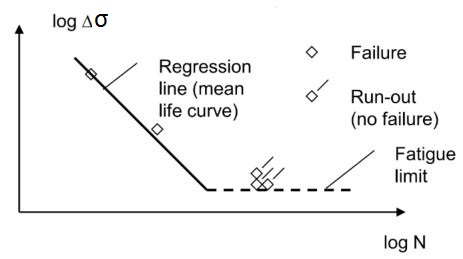
\includegraphics[scale=1]{figures/sn}
\caption[$\; \:$Example of an SN curve]{Example of an SN curve, \cite{fatigue2016} }
 \label{fig:sn}
\end{wrapfigure}

Where N is the number of cycles before failure, $\Delta \sigma$ is the stress range, m is an exponent and c is a constant. \cite{dnvfatigue} elaborates that by subtracting two standards deviations, the SN-curve represents 97.6\% of survival. \newline
\newline
For the low cycle fatigue, the material undergoes plastic deformation. For marine structure applications, the stress is usually in the high cycle fatigue range. If the stress range is sufficiently low, fatigue life can approach "infinite". A stress range of this nature is called the fatigue limit and only applies in non-corrosive environments. \\\\ The damage done by one cycle is usually close to insignificant, and undetectable by instruments. Failure due to fatigue is a result of the cumulative damage induced by the cyclic loading. For marine structures, load from waves, current, motions, and vortex-induced vibrations may cause severe damage. Fatigue damage can be divided into three stages:
 \begin{itemize}
     \item Crack initiation, $N_i$
     \item Crack growth, $N_g$
     \item Failure
 \end{itemize}
 This means that the fatigue life can be calculated as:
 \begin{equation}
     N=N_i+N_g
 \end{equation}
 
\subsection{Irregular Loading}
For marine structures, irregularly cyclic loading is common, see Figure \ref{fig:irr}, where the amplitude and frequency vary over time. The lifespan for a typical specimen in the offshore industry is 20 years with an average frequency at 16 1/s. To make the design process manageable, this has to be reduced to a more practical format.  

\begin{figure}[H]
\centering
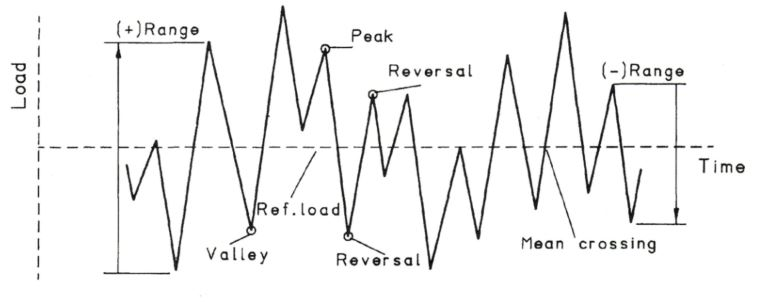
\includegraphics[scale=0.8]{figures/irr}
\caption[$\; \:$Example of irregular loading]{Example of irregular loading, \cite{fatigue2016} }
 \label{fig:irr}
\end{figure}

In Figure \ref{fig:irr}, a few concepts of irregular loading are defined:
\begin{itemize}
\item Reversal - Where the first derivative changes sign
    \item Peak - Where the first derivative changes from a positive to a negative sign
    \item Valley - Where the first derivative changes from negative to a positive sign
    \item Range - Difference between a peak and a valley
    \item Mean crossing - number of time the load-time history crosses the mean load level (normally only crossings with positive first derivatives are counted)
    \item Bandwidth - Ratio of mean crossings with positive slopes to the number of peaks or valleys. 
\end{itemize}
 
\subsection{Rainflow Counting}
\label{sec:rainflow}
\begin{wrapfigure}{r}{0.5\textwidth}
    \vskip -1.0 cm 
    \centering
    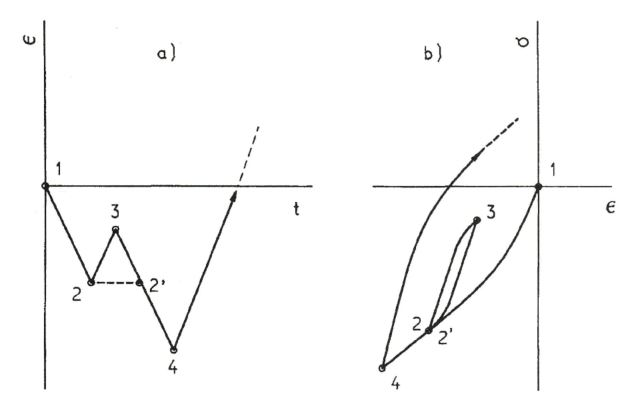
\includegraphics[scale=0.6]{figures/count}
\caption[$\; \:$Cyclic load and stress-strain response]{(a) Cyclic load, (b) Stress-strain response,   \cite{fatigue2016} }
 \label{fig:count}
\end{wrapfigure}
There are several ways of counting cycles, and Rainflow Counting is one of them. The name of this method stems from the thought of rain falling on the roof of a pagoda (Chinese architecture). In this procedure, the reversals are counted in accordance with the stress-strain response. The procedure can be seen in Figure \ref{fig:count}, where the cycle from 2-3-2' does not affect the rest of the stress-strain cycle. Each time a loop is completed, a cycle count is made, so that the counting of the cycles reflects the response of the material. The fatigue damage caused by a closed loop in the irregular amplitude loading is, according to this counting method, the same as one cycle in a constant amplitude test. Half cycles cannot be paired up with other half cycles, so the damage they do on the structure is not counted in this method. However, in a realistic case, there are few half cycles. Due to its versatility, the Rainflow method is considered superior to other counting methods. \\\\
The Rainflow Counting algorithm is illustrated in \ref{fig:pagoda}. Begin at the first valley. If the next valley is deeper or equal to the first one, the rainflow stops here and a cycle is counted, (see point 5 in Figure \ref{fig:pagoda}). If the valley is not deeper than the first one, the flow proceeds to the next valley, (see point 3 in Figure \ref{fig:pagoda}). The rain-flow is also considered to stop if it meets another flow from above, (see point 2' in Figure \ref{fig:pagoda}) When one rainflow has stopped, proceed to the next valley and repeat the procedure. After completion of counting of valleys, the same procedure is performed on the peaks. The results from the Rainflow Counting can be gathered in a histogram that easily shows the number of cycles for different classes. \begin{figure}[H]
\centering
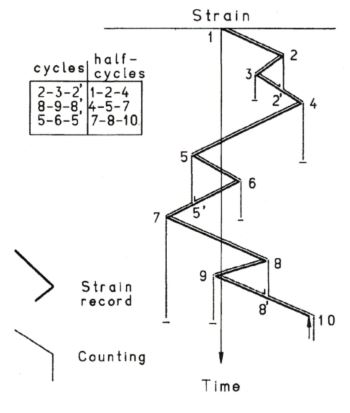
\includegraphics[scale=0.9]{figures/pagoda}
\caption[$\; \:$Rainflow Counting]{Rainflow Counting with illustration of the Chinese pagoda origin,   \cite{fatigue2016} }
 \label{fig:pagoda}
\end{figure}
\noindent In this master thesis, Rainflow Counting was utilized by using a module in Pyhton called rainflow.py. According to \cite{rf}, the module implements ASTM E1049-85 rainflow cycle counting
algorithm, and is meant for fatigue analyses. The function rainflow.count\_cycles takes in a 1D array of numbers and returns a sorted list of the load ranges and the corresponding
number of cycles.

\subsection{Cumulative Damage}
Several methods can be applied to calculate the cumulative damage due to irregular amplitude cyclic loading. The Miner-Palmgren approach has proven to be as good as other methods and is extremely simple. The Miner-Palmgren theory assumes that the damage is constant during a given stress range. The Miner-Palmgren expression:
\begin{equation}
    D=\sum_i \frac{n_i}{N} 
    \label{eq:MP}
\end{equation}
where D is the accumulated damage, $n_i$ is the number of cycles with a certain stress range experienced by the structure and N is the fatigue life of at that stress range.\newline
\newline
According to \cite{riserfat}, the fatigue criterion which shall be satisfied is expressed as:
\begin{equation}
    D \cdot \text{DFF} \leq 1.0
\end{equation}
Where D is the accumulated damage and DFF is the Design Fatigue Factor.\\\\ Table \ref{table:dff} show the different Design Fatigue Factors recommended by \cite{riserfat}. 

\begin{table} [H]
\centering
\begin{tabular}{ |c|c|c|}
\hline
\multicolumn{3}{|l|}{\hspace{0.8cm}Safety Class}\\
 \hline
 \hline
Low & Medium & High \\
3.0 & 6.0 & 10.0\\
 \hline
\end{tabular}
\caption{Design Safety Facros (DFF) for different safety classes  recomended by \cite{riserfat}.}
\label{table:dff}
\end{table}
\subsection{Mean Stress Correction}
\label{sec:meanstress}
According to \cite{Savik2016}, fatigue tests of steel or copper wires are often done with constant mean stress or the R-ratio constant and always positive to avoid compression. Testing in tension-tension mode normally has a R-ratio of 0.1-0.5, and SN-diagrams deviating from the given R-ratio are often not obtainable.  The applied stress range can be calculated for a given R-ratio as:

\begin{equation}
    \Delta \sigma = 2 \bar{\sigma} \frac{1-R}{1+R}
\end{equation}
A Haigh diagram gives the relationship between the stress range ($\Delta \sigma$) and the mean stress ($\bar{\sigma}$).  Fatigue tests at given R-ratios form a straight line in the Haigh diagram, as illustrated in Figure \ref{fig:gerber}. To remedy the limitation that  SN curves are only available for a certain R-ratio, Goodman, Gerber or Söderberg assumptions can be employed to transform between different mean stresses. They are described by the following expressions:\newline
\newline
\begin{wrapfigure}{r}{0.5\textwidth}
    \vskip -1.0 cm 
    \centering
   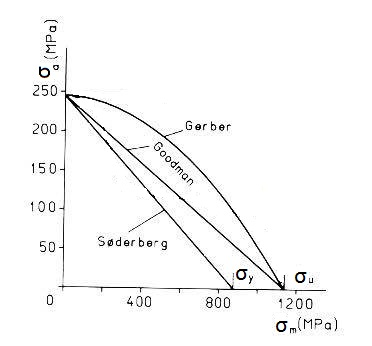
\includegraphics[scale=0.8]{figures/soder.PNG}
\caption[$\; \:$Goodman, Gerber and Söderberg relations]{Goodman, Gerber and Söderberg relations, adapted from \cite{fatiguehand} }
 \label{fig:gerber}
\end{wrapfigure}
\noindent Goodman assumption:
\begin{equation}
    \Delta \sigma_0 = \frac{\Delta \sigma}{1-(\frac{\bar{\sigma}}{\sigma_u})}
\end{equation}

\noindent Gerber assumption:
\begin{equation}
    \Delta \sigma_0 = \frac{\Delta \sigma}{1-(\frac{\bar{\sigma}}{\sigma_u})^2}
\end{equation}

\noindent Söderberg assumption, \cite{fatiguehand}:
\begin{equation}
    \Delta \sigma_0 = \frac{\Delta \sigma}{1-(\frac{\bar{\sigma}}{\sigma_y})}
\end{equation}

\noindent where $\Delta \sigma_0$ is the stress range at zero mean stress, $\Delta \sigma$ is the calculated stress range, $\bar{\sigma}$ is the mean stress level, $\sigma_u$ is the ultimate stress level of the material, and $\sigma_y$ is the yield stress level of the material. The Goodman, Gerber, and Söderberg assumptions can also be seen in Figure \ref{fig:gerber}. 

\subsection{Fatigue of Dynamic Power Cables}
\noindent \cite{Nasution2013} states that when the cable is in operation, it experiences loads from gravity, the motions of the floating vessel, and from the sea. The cable experiences a mean global tension and torque due to gravity. Surge and heave motions induce dynamic tensile and torque, while pitch and roll motions give a dynamic curvature of the cable. This can be seen in Figure \ref{fig:float}. 

\begin{figure}[H]
\centering
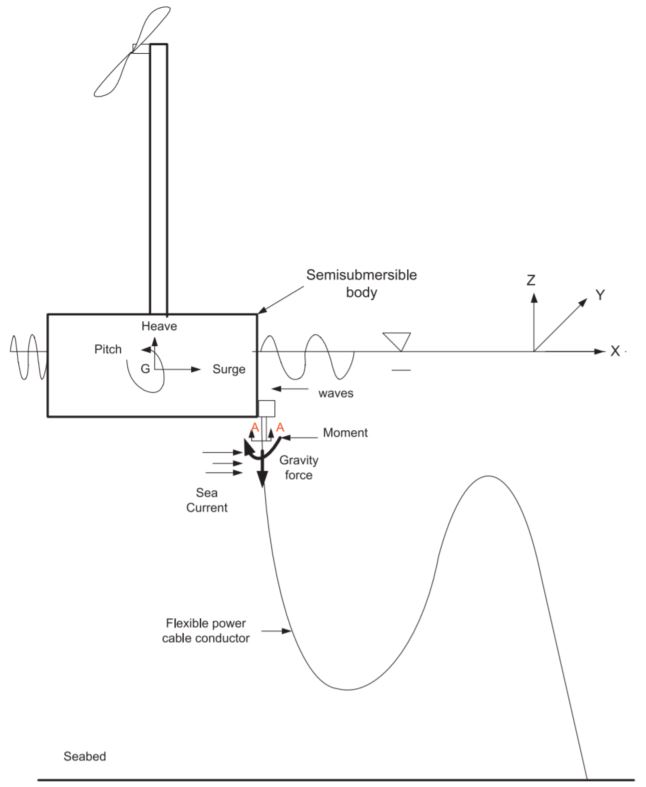
\includegraphics[scale=0.7]{figures/float}
\caption[$\; \:$Dynamic flexible power cable attached to semi-submersible wind turbine]{Dynamic flexible power cable attached to semi-submersible wind turbine, \cite{Nasution2013}}
 \label{fig:float}
\end{figure}
\noindent \cite{YangShun-Han2017} states that fatigue life is an important parameter in determining service life for a subsea a power cable. \cite{Thies2012} explains that power cables can be used in static applications, where it is connected to a fixed structure, or dynamic application where they have to withstand significant cyclic loading. Due to this, dynamic power cables are subjected to fatigue failure.\\\\
There are mainly three causes of mechanical failure in marine power cables applied to marine energy applications, taken from \cite{Thies2012}:

\begin{itemize}
    \item Maximum axial tension
    \item Over bending
    \item Fatigue under extreme cyclic loads
\end{itemize}

\noindent According to \cite{Karlsen2010}, the individual wires and the intersections between them is what determines the fatigue properties of a copper conductor. R-ratio of loading and wire interaction have been recognized as relevant factors to fatigue life in copper conductors. Fretting fatigue (fatigue due to oscillating load on a junction between two components \cite{Hills1994}) is identified as one of the dominating mechanisms in multi-layer stranded steel wires. Friction force increases with increasing lay angle and friction coefficient for the material. The copper conductors do not only have contact between conductor surfaces, but also with the protecting sheath around the conductors, giving a complex stress model.

\subsubsection{Fatigue of Copper Conductors}
\label{sec:fatcop}
According to a study done by \cite{Nasution2013}, when testing individual wires as well as a full cross-section of a three-phase 95mm$^2$, all failures occurred in the inner layer for the cross-section bent over a bell mouth. Also, individual wires from the outer layer of the cross-section were tested in controlled tension-tension loading. Here, all initiation of crack growth happened within or at the edge of the trellis contact area, that has been deformed due to the compacting process of the cable. The study concluded that the difference in fatigue life between layers is due to the variance of surface irregularities. Another study, performed by \cite{NASUTION2014} states that the first fatigue failure for a copper conductor subjected to tension-tension fatigue happens in the outer layer. this indicates that the fatigue performance is governed by local effects due to surface irregularities of the different layers. \newline
\newline
\subsubsection{Analytical Model} \cite{s300} developed an analytical model for stress variation in individual wires in the conductor cross-section. This model applies for conductors exposed to static and dynamic tension in combination with dynamic curvature. The stress variation can be calculated as:   
\begin{equation}
    \Delta \sigma = \Delta \sigma_T + \Delta \sigma_{tc} + \Delta \sigma_{nc} + \Delta \sigma_{f}
    \label{eq:stressvariation}
\end{equation}
\noindentWhere $\Delta \sigma_T$ is the stress range due to dynamic tension, $\Delta \sigma_{tc}$ is the stress range from transverse curvature of the wire, $\Delta \sigma_{nc}$ is the stress range from normal curvature of the wire and $\Delta \sigma_{f}$ is the stress range from friction. By looking at a point with the polar coordinate angle $\psi = 0$, Expression \ref{eq:stressvariation} can be reduced to:
\begin{equation}
    \Delta \sigma = (\Delta \sigma_f + \Delta \sigma_{T})\cdot \text{SCF} + \Delta \sigma_{nc}
    \label{eq:stressvariationred}
\end{equation}Where SCF is the stress concentration factor. \\\\The stress variation in the individual wires due to dynamic tension can be found from:
\begin{equation}
    \Delta \sigma_T^i = E \cos^2 \alpha_i \frac{\Delta T}{E A_{full}} 
    \label{eq:sigmaT}
\end{equation}
\noindent Where E is the Young's modulus of the material, $\Delta T$ is the tension range and $EA_{full}$  is the axial stiffness of the full cross-section of the conductor and can be found from:
\begin{equation}
    EA_{full}=EA \left( 1+\sum_{i=1}^m n_i \cos^3\alpha_i \right)
\end{equation}
\noindent Where EA is the axial stiffness of each wire, $n_i$ is the number of wires in layer i, and $\alpha_i$ is the lay angle of layer i. \newline
\newline
The bending stress range from normal curvature of the wires for small lay angles can be approximated as:
\begin{equation}
    \Delta \sigma_{nc} = R_{nominal} E \cos^2 \alpha_i \cos2 \alpha_i \Delta \kappa \cos \Psi \approx R_{nominal}E \Delta \kappa
\end{equation}
where $\Delta \kappa$ is the curvature range and $\Psi$ is the polar coordinate angle defining the helix position (assuming $\psi=0$). \newline
\newline
The friction stress range will be the smallest stress range from either the plane surfaces remain plane solution or maximu mallowed due to friction between the interfaces:
\begin{equation}
    \Delta \sigma_f^i =\text{min}\left(E \cos^2 \alpha_i R_i \Delta \kappa , \frac{\pi R_i \tau_i}{\sin \alpha_i A_i}\right)
\end{equation}
where $R_i$ is the helix radius of the layer i, and $\tau_i$ is the friction force per unit length, and can be determined by:
\begin{equation}
    \tau_i \cong E \epsilon_c \mu \left( \sum_{j=i+1}^m \frac{n_j A_j \cos^2 \alpha_j \sin^2 \alpha_j }{n_i R_i} + \sum_{j=i}^m \frac{n_j A_j \cos^2 \alpha_j  \sin^2 \alpha_j}{n_j R_i}\right)
\end{equation}
where $\mu$ is the coefficient of friction and $\epsilon_c$ can be found from:
\begin{equation}
    \epsilon_c =\frac{T}{EA_{full}}
    \label{eq:stressvariation2}
\end{equation}